\documentclass[../main.tex]{subfiles}


\begin{document}
\section{Data read in system}
	The first challenge part of the project was to create a data read in system in order to allow data analysis. The data files come in the form on .csv files which has
	the data structure seen in Figure \ref{datastructure}.
	\begin{figure}[!h]
	  \centering
	  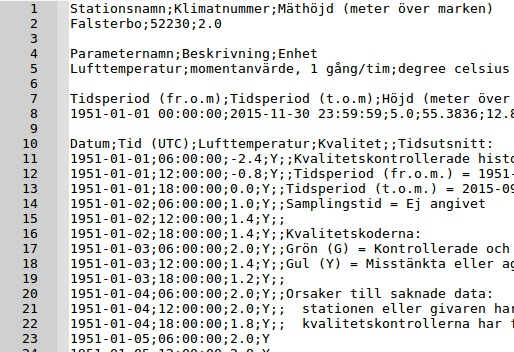
\includegraphics[width = \textwidth]{datastructure.jpg}
	  \caption{Data structure of the files used for analysis.}
	  \label{datastructure}
	 
	\end{figure}\noindent
	The first couple of lines consists of information which is irrelevant for reading in, which is why a for loop was used in order to skip the first lines until it reaches 
	the first data point, which can be identified by its ``year-month-day;hour:minute:second;temperature`` format.
	\\\\
	In order to obtain the information in each data point it was first split into three separate strings at each '';``. In the next step the ``year-month-day'' string was split 
	further at each ``-'' and stored into separate vectors. The same was done to the ``hour:minute:second'' string for each ``:'' and the hour was stored in a 
	vector (the data points contains no minutes or seconds and are thus not saved).
	

	\vspace{2mm}
	\begin{lstlisting}[frame=single] 
for (k = 0; (unsigned)k < (year.size()-1); k++) { 
	if (temperature.at(k) > hottest){ 
		hottest = temperature.at(k);
		hottestDay = day.at(k);
		hottestMonth = month.at(k);
	}
}
	\end{lstlisting}
\end{document}